\chapter{Anwendungen von Algorithmen}
%Grundeinleitung
In den vorherigen Kapiteln wurden die Grundlagen der Funktionsprinzipien von Algorithmen zur Pfadplanung erl"autert, sodass man einen groben "Uberblick "uber jene bekommt. Doch wozu nutzt man konkret dieses Algorithmen? Diese Pfadplanungsalgorithmen werden verwendet, um Probleme zu l"osen, bzw. um Probleme von Maschinen l"osen zu lassen, die so komplex sein k"onnen, dass Menschen Probleme haben diese ohne Hilfsmittel zu l"osen.\\
Im Folgenden sind einige Beispiele zu Anwendungen von Algorithmen zu Pfadplanung zusammengetragen und erl"autert.

\section{Anwendungen mit diskretem Zustandsraum}
Wie in Kapitel \ref{Kapitel 4.3} zur disktete Pfadplanung beschrieben, ist der Zustandsraum bei diskreten Zust"anden endlich oder abz"ahlbar unendlich. Diese Parameter sind z.B. f"ur das Rubik's Cube R"atsel zutreffend (siehe Abb. \ref{Abb. 5.1}), bei dem es ebenso einen endlichen Zustandsraum und einen endlichen Aktionsrahmen gibt. Der Zustandsraum ist hierbei die Summe aller Zust"ande, die der W"urfel annehmen kann, also jegliche m"ogliche Farbverteilung. Der Aktionsrahmen ist die Menge aller Richtungen, in die man jedes Element drehen kann.\\ Nun wird bei einem Rubik's Cube kein Pfad im klassischen Sinne geplant, jedoch handelt es sich auch hier um ein diskretes Problem.\\
\begin{figure}
	\centering
	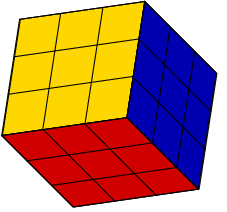
\includegraphics[width=0.4\linewidth]{images/img229}
	\caption{in Anlehnung Abb. 1.1 von \cite[~S. 5]{Lav06}: Rubik's Cube.}
	\label{Abb. 5.1}
\end{figure}

Bei der n"achsten Anwendung, den Bewegungen eines Roboters oder einer K"unstlichen Intelligenz auf einem 2D Netz, wird nun aber tats"achlich ein Pfad geplant. Dies passiert beispielsweise in Computerspielen wie Echtzeit-Strategiespielen, in denen eine Figur von ihrem aktuellen Standpunkt zu einem Ort gelangen muss, der ihr zugewiesen wird. Hier kommt der Pfadplanungsalgorithmus zum Einsatz.\\
%s27ff
\section{Anwendungen zur Planung mit kontinuierlichem Zustandsraum}
Wie in Kapitel \ref{Kapitel 4.2} schon angeschnitten klassifiziert man bei den Algorithmen zur Planung mit kontinuierlichem Zustandsraum zwischen drei verschiedenen Rubriken, die unterschiedliche Anwendungsbereiche haben, auf die im Folgenden einzeln eingegangen wird.
\subsection{Anwendungen zur Planung mit allen Umgebungsinformationen vorhanden}
Ein gutes Beispiel f"ur Anwendungen zur Planung, bei der alle Umgebungsinformationen vorhanden sind, ist das bekannte Piano Mover's Problem. Ein Piano Es existiert kein Netz, auf dem das Piano bewegt werden kann. Es gibt einen "uberabz"ahlbar unendlichen Zustandsraum, jedoch ist die Umgebung genau bekannt.\\
Eine weitere praxisn"ahere Anwendung ist das automatische An- und Abmontieren eines Scheibenwischermotors an ein Auto, wie in Abb. \ref{Abb. 5.2} dargestellt.
\begin{figure}
	\centering
	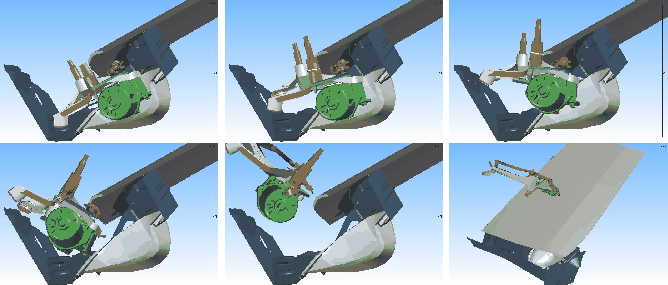
\includegraphics[width=0.7\linewidth]{images/img231}
	\caption{Abb. 1.3 von \cite[~S. 7]{Lav06}: Eine Auto-Montierungsaufgabe, die beinhaltet, dass ein Scheibenwischermotor an ein Auto angebracht oder entfernt werden soll.}
	\label{Abb. 5.2}
\end{figure}

Eine Software muss entscheiden, ob der Scheibenwischermotor An- und abmontiert werden kann, oder nicht. Das fr"uher zeit- und kostenintensive Entwickeln des Designs wird nun mit Software vereinfacht, indem CAD Modelle manipuliert werden. Auch hier hat man einen "uberabz"ahlbar unendlichen Zustandsraum und alle Umgebungsinformationen sind bekannt.
%part 2
\subsection{Anwendungen zur Planung mit Unsicherheit}
Bei der Planung mit Unsicherheit (engl. planning under uncertanty), auch decision-theoretic planning genannt, interferieren Ungewissheiten im Allgemeinen mit 2 Aspekten des Planens. Diese beiden Aspekte sind Vorhersehbarkeit und Wahrnehmung.\\
Die Vorhersehbarkeit ist in dem Sinne durch die Unsicherheiten beeintr"achtigt, dass nicht bekannt ist, was passieren wird, gewisse Aktionen ausgef"uhrt werden und die Wahrnehmung ist durch die Unsicherheiten beeintr"achtigt, da der aktuelle Status, bzw. die aktuelle Position nicht bekannt ist. Denn den Status erh"alt man aus den Ausgangsbedingungen, den Sensoren und den Informationen über die vorangegangenen Aktionen.\\
Ein Beispiel f"ur eine solche Anwendung ist der Tesla Autopilot oder Autonomes Fahren im Allgemeinen. Hier bewegt sich das Auto nicht über ein festes 2D Netz, sondern durch die unvorhersehbare Realit"at. Der Bordcomputer des Autos nimmt durch seine Sensoren und eventuelle Au"senkameras seine Umgebung war und versucht durch diese und GPS-Daten seinen Status bzw. seine aktuelle Position herauszufinden. Da sich jedoch die Umgebung stets ver"andert und der Verhalten der anderen Verkehrsteilnehmer nicht vorhersagbar ist, kommt die Unsicherheit ins Spiel.
Dies l"asst sich auf die Navigation von allen mobilen Robotern "ubertragen.
Da der aktuelle Status nie gewiss sein kann, wird mit allen verf"ugbaren Informationen versucht, den Status so genau wie m"oglich zu bestimmen.
%(s.25) Part 3
\subsection{Anwendungen zur Planung mit Bewegungseinschr"ankungen}
Bei Anwendungen zur Planung mit Bewegungseinschr"ankungen (engl. planning under differential constraints) hat man ebenfalls einen Zustandsraum von "uberabz"ahlbar unendlich, zus"atzlich muss aber noch beachtet werden, dass der schnellste Pfad, der errechnet w oft durch Bewegungseinschr"ankungen nicht umgesetzt werden kann. In der Robotik entstehen diese Bewegungseinschr"ankungen h"aufig durch die Kinematik und Dynamik der Roboter selbst.\\
Auch hier kann gut Auto als Beispiel herhalten. Ein Auto kann nicht seitw"arts fahren. Wenn es also seitlich neben einer Parkl"ucke steht und man den Einparkassistenten das Auto einparken lassen will, w"are der k"urzeste Pfad seitw"arts zu fahren. Da die nicht m"oglich ist, muss das bei der Pfadplanung ber"ucksichtigt werden(siehe Abb. \ref{Abb. 5.3}).
\begin{figure}
	\centering
	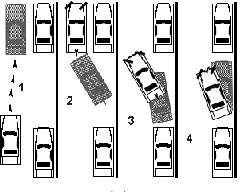
\includegraphics[width=0.5\linewidth]{images/img239}
	\caption{in Anlehnung an Abb. 1.11 von \cite[~S. 15]{Lav06}}
	\label{Abb. 5.3}
\end{figure}

%s26 Part IV